\documentclass[11pt]{article}

\usepackage[utf8]{inputenc}
\usepackage{fancyhdr}
\usepackage{hyperref}
\usepackage{graphicx}

\graphicspath{ {images/} }
 
\pagestyle{fancy}
\fancyhf{}
\lhead{University of the Witwatersrand}
\rfoot{School of Computer Science and Applied Mathematics}
\pagenumbering{roman}
\fancyfoot[R]{\thepage}

\begin{document}
\begin{page}

\newcommand{\HRule}{\rule{\linewidth}{0.3mm}} % Defines a new command for the horizontal lines, change thickness here
\renewcommand\section{\@startsection{section}{1}{\z@}%
                                  {-3.5ex \@plus -1ex \@minus -.2ex}%
                                  {2.3ex \@plus.2ex}%
                                  {\normalfont\large\bfseries}}
\setlength{\parindent}{0pt}

\center % Center everything on the page
 
%----------------------------------------------------------------------------------------
%	HEADING SECTIONS
%----------------------------------------------------------------------------------------

\textsc{\LARGE University of the Witwatersrand}\\[1.5cm] % Name of your university/college
\textsc{\Large School of Computer Science and Applied Mathematics}\\[0.5cm] % Major heading such as course name

%----------------------------------------------------------------------------------------
%	TITLE SECTION
%----------------------------------------------------------------------------------------

\HRule \\[0.4cm]
{ \huge \bfseries COMS3007: Machine Learning Assingment}\\[0.4cm] % Title of your document \\
  \large 13 May 2016
\HRule \\[1.5cm]
 
%----------------------------------------------------------------------------------------
%	AUTHOR SECTION
%----------------------------------------------------------------------------------------
\begin{minipage}{1\textwidth}
	\Large \emph By Chalom, J. (711985)\\
\end{minipage}


\vfill % Fill the rest of the page with whitespace

\end{page}

\begin{page}

\clearpage
\setcounter{page}{1}
\tableofcontents
\clearpage
\pagenumbering{arabic}

\section{Purpose}
The purpose of my assignment is to use machine learning in order to correctly classify hand written digits as their corresponding ASCII equivalents, or at least predict within an acceptable order of magnitude. These sets of experiments will hopefully show that machine learning can be applied to the field of optical character recognition.

\section{Tools Used}
I made used of the node.js framework for my coding and scripting of the various experiments. I used the Synaptic neural network library for node.js. This library was capable of handling constructing the given dimensions of a network, changing relevant values, randomising the data and calculating the error during training. \url{http://synaptic.juancazala.com/}

\section{Dataset Used}
I made use of the MNIST database. This is a large database of hand written digits which has been compiled by taking a combination of two databases of hand written digits in the United States. The website for this database can be found here: \url{http://yann.lecun.com/exdb/mnist/} \\

\noindent This database has a very large training set of 60 000 examples and a set of 10 000 test examples. All the images are normalised, and centred in the same fixed size of 28x28 pixels. The images have all been pre-processed.

\noindent I used the mnist library for node.js to help me load the database into Synaptic. It can be found here: https://github.com/cazala/mnist \\\\

\noindent Using this library I was able to specify the number of training samples and testing samples I wanted. No two sets are identical. I specified 700 training examples and 20 testing examples. \\\\

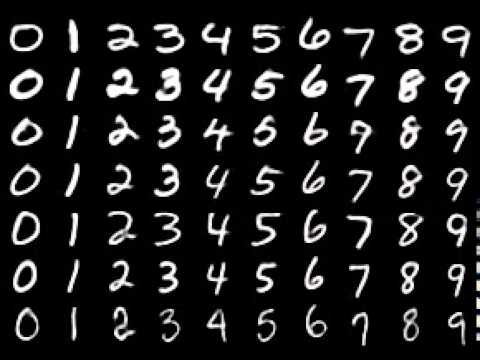
\includegraphics[scale=0.7]{1}\\
An example of the data used (several sets of samples compiled together) \\
Source: \url{https://github.com/cazala/mnist/}\\

\noindent My neural networks all had 784 input nodes (which correspond per pixel to the input image samples) and 10 output nodes (which correspond to the digits 0-9) as my attributes of classification. My networks, setup using Synaptic js accept a 784 length array of values (floats) and outputs a 10 length array of values (floats). I run the test data on the network after training and round the output values to the nearest integer after the network has completed running the data. \\\\

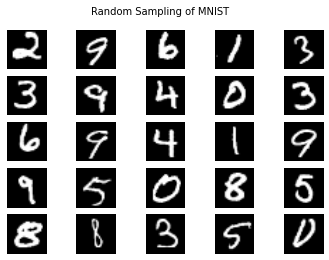
\includegraphics{2}\\
This is an example of a randomly sampled data:\\
Source: \url{http://ampcamp.berkeley.edu/6/exercises/} 


\section{Algorithms Used}
\emph Note: See results for the error returned on the test set.\\
 
\noindent Synaptic runs multiple iterations of each network when training. Each iteration randomises the data so the error will have variation. On all experiments I ran 10 iterations (detailed in Results).\\
\\
\noindent \textbf{Experiment 1:} Neural network with one hidden layer with 100 nodes and learning rate of 0.3\\\\
\textbf{Experiment 2:} Neural network with two hidden layers with 50 nodes on each layer and a learning rate of 0.3\\\\
\textbf{Experiment 3:} Neural network with three hidden layers with 25 nodes on each layer and a learning rate of 0.3\\\\
\textbf{Experiment 4:} Neural network with three hidden layers with 50 nodes on each layer and a learning rate of 0.3\\\\
\textbf{Experiment 5:} Neural network with two hidden layers with 50 nodes on each layer and a learning rate of 0.2\\\\
\textbf{Experiment 6:} Neural network with three hidden layers with 20 nodes on each layer and a learning rate of 0.2\\\\
\textbf{Experiment 7:} Neural network with three hidden layers with 25 nodes on layer 1, 50 modes on layer 2, 25 nodes on layer 3 and a learning rate of 0.3\\\\
\textbf{Experiment 8:} Logistic Regression with a learning rate of 0.2. This is to see if this method is viable to use. Had to use another Node.JS library called machine learning.\\\\

\section{Results}
The results here are pulled from the raw output that Synaptic returned when it was run at each configuration. One test set from each experiment is also given. Both the expected result and actual values before being normalised are shown.\\

\noindent \textbf{Experiment 1:} \\
Time Taken: 18 minutes to run\\

\noindent iteration 1 error 25.21775948402851 rate 0.3\\
iteration 2 error 20.9936226883679 rate 0.3\\
iteration 3 error 19.386880788481065 rate 0.3\\
iteration 4 error 18.567642667973264 rate 0.3\\
iteration 5 error 16.70118832915488 rate 0.3\\
iteration 6 error 16.93568631810135 rate 0.3\\
iteration 7 error 15.122139345854992 rate 0.3\\
iteration 8 error 17.135472581921587 rate 0.3\\
iteration 9 error 16.900383217441735 rate 0.3\\
iteration 10 error 16.45530516020001 rate 0.3\\\\

\noindent \textbf{Example Test Set:}\\
Result using testSet[10]: Expected Result After Rounding (0,0,0,0,1,0,0,0,0,0)\\\\

\noindent 4.442733281764681e-11,\\
  8.2302476995108e-13,\\
  1.5367202058008483e-22,\\
  0.9985015298088129,\\
  4.204662258786807e-10,\\
  0.0007053373062841791,\\
  8.933665406962743e-23,\\
  1.574202993533067e-10,\\
  1.4744065920990558e-22,\\
  0.000004165508043373923\\
\\
\noindent \textbf{Experiment 2:} \\
Time Taken: 9 minutes to run\\

\noindent iteration 1 error 13.579141802549136 rate 0.3\\
iteration 2 error 13.918781153165188 rate 0.3\\
iteration 3 error 13.68188869593232 rate 0.3\\
iteration 4 error 13.966400906380482 rate 0.3\\
iteration 5 error 13.705195781711677 rate 0.3\\
iteration 6 error 14.120244682331546 rate 0.3\\
iteration 7 error 13.836942593523935 rate 0.3\\
iteration 8 error 13.531639258263477 rate 0.3\\
iteration 9 error 13.77157524266658 rate 0.3\\
iteration 10 error 13.750266157976949 rate 0.3\\\\

\noindent \textbf{Example Test Set:}\\
Result using testSet[4]: Expected Result After Rounding (0,1,0,0,0,0,0,0,0,0)\\\\

\noindent  0.00016379264818057416,\\
  0.9984374585230067,\\
  0.00016796313619995274,\\
  0.00015203924039180894,\\
  0.00015521953214318873,\\
  0.00016199101297130714,\\
  0.0001614617975365281,\\
  0.00015448652475491586,\\
  0.00016490551683624605,\\
  0.00016614082681160026\\\\

\noindent \textbf{Experiment 3:} \\
Time Taken: 4 minutes to run\\

\noindent iteration 1 error 7.1118987482174685 rate 0.3\\
iteration 2 error 7.304910698299639 rate 0.3\\
iteration 3 error 7.296114225371919 rate 0.3\\
iteration 4 error 7.057774875964977 rate 0.3\\
iteration 5 error 7.323047640926627 rate 0.3\\
iteration 6 error 7.16302385976031 rate 0.3\\
iteration 7 error 7.276213386307813 rate 0.3\\
iteration 8 error 7.037327285923723 rate 0.3\\
iteration 9 error 7.283030418143739 rate 0.3\\
iteration 10 error 7.154851736553406 rate 0.3\\\\

\noindent \textbf{Example Test Set:}\\
Result using testSet[4]: Expected Result After Rounding (0,0,0,0,0,0,0,0,1,0)\\\\

\noindent 0.006438510929018079,\\
  0.004884896010748979,\\
  0.010265013305559931,\\
  0.007500203817356501,\\
  0.008178200371097271,\\
  0.0037174246798148906,\\
  0.005440941570821145,\\
  0.002784100761579707,\\
  0.9678857620887612,\\
  0.008424696901711274\\

\noindent \textbf{Experiment 4:} \\
Time Taken: 10 minutes to run\\

\noindent iteration 1 error 13.78893222831105 rate 0.3\\
iteration 2 error 13.962875306571101 rate 0.3\\
iteration 3 error 13.725664067343615 rate 0.3\\
iteration 4 error 13.792150437515117 rate 0.3\\
iteration 5 error 13.639755810528895 rate 0.3\\
iteration 6 error 13.662269808140653 rate 0.3\\
iteration 7 error 13.684097094291813 rate 0.3\\
iteration 8 error 13.771657098278137 rate 0.3\\
iteration 9 error 14.011845114495829 rate 0.3\\
iteration 10 error 13.575661104186732 rate 0.3\\\\

\noindent \textbf{Example Test Set:}\\
Result using testSet[14]: Expected Result After Rounding (0,0,0,1,0,0,0,0,0,0)\\\\

\noindent 0.00016190260722350215,\\
  0.00015854811374045567,\\
  0.00017207927367805036,\\
  0.9984397634630661,\\
  0.00014953665665581937,\\
  0.00015295836713093413,\\
  0.00016378306908067068,\\
  0.00016903774734393327,\\
  0.00016035204142152975,\\
  0.00015883026108401237\\
\\
\noindent \textbf{Experiment 5:} \\
Time Taken: 5 minutes to run\\

\noindent iteration 1 error 9.099641366585107 rate 0.2\\
iteration 2 error 9.378963093104808 rate 0.2\\
iteration 3 error 9.297211484789804 rate 0.2\\
iteration 4 error 9.29961398543107 rate 0.2\\
iteration 5 error 9.272032419591685 rate 0.2\\
iteration 6 error 9.343386069684948 rate 0.2\\
iteration 7 error 9.21525966473154 rate 0.2\\
iteration 8 error 9.316787676939901 rate 0.2\\
iteration 9 error 9.172782970605343 rate 0.2\\
iteration 10 error 9.202069212000243 rate 0.2\\\\

\noindent \textbf{Example Test Set:}\\
Result using testSet[3]: Expected Result After Rounding (0,0,0,0,0,0,0,0,0,1)\\\\

\noindent 0.001929271257700453,\\
  0.0013540966164573304,\\
  0.002791321851632145,\\
  0.001983607742412473,\\
  0.001775797737041715,\\
  0.002283297623056343,\\
  0.002660004042935651,\\
  0.001536455957136727,\\
  0.0015606054810134232,\\
  0.9859943961815629\\
\\
\noindent \textbf{Experiment 6:} \\
Time Taken: 2 minutes to run\\

\noindent iteration 1 error 4.578398747115859 rate 0.2\\
iteration 2 error 4.662957558912961 rate 0.2\\
iteration 3 error 4.647463617041337 rate 0.2\\
iteration 4 error 4.708482887577781 rate 0.2\\
iteration 5 error 4.632380940780409 rate 0.2\\
iteration 6 error 4.648153171528649 rate 0.2\\
iteration 7 error 4.554928564341489 rate 0.2\\
iteration 8 error 4.685728993835576 rate 0.2\\
iteration 9 error 4.651785892758141 rate 0.2\\
iteration 10 error 4.6209499777439484 rate 0.2\\\\

\noindent \textbf{Example Test Set:}\\
Result using testSet[4]: Expected Result After Rounding (1,0,0,0,0,0,0,0,0,0)\\\\

\noindent 0.9028138579446788,\\
  0.036619873615160385,\\
  0.021265482921776616,\\
  0.013378610101175458,\\
  0.02477443816979929,\\
  0.012536869749274596,\\\\
  0.012076260935591398,\\
  0.01099683744627199,\\
  0.07401282476211142,\\
  0.054308164482469286\\
\\
\noindent \textbf{Experiment 7:} \\
Time Taken: 3 minutes to run\\

\noindent iteration 1 error 7.115278691252323 rate 0.3\\
iteration 2 error 7.238494326127107 rate 0.3\\
iteration 3 error 7.229231318797966 rate 0.3\\
iteration 4 error 7.038426626866396 rate 0.3\\
iteration 5 error 7.0913088782913904 rate 0.3\\
iteration 6 error 7.211607855291496 rate 0.3\\
iteration 7 error 7.191426156662719 rate 0.3\\
iteration 8 error 7.136818906956898 rate 0.3\\
iteration 9 error 7.0409793129796565 rate 0.3\\
iteration 10 error 7.154835185463085 rate 0.3\\\\

\noindent \textbf{Example Test Set:}\\
Result using testSet[1]: Expected Result After Rounding (1,0,0,0,0,0,0,0,0,0)\\\\

\noindent 0.9121143456794434,\\
  0.010713645792990851,\\
  0.006044436783441403,\\
  0.008017351664189981,\\
  0.006693299596284033,\\
  0.009055802293537644,\\
  0.007900081622224636,\\
  0.008220055576803028,\\
  0.0031237307501818766,\\
  0.006684781607826813\\
\\
\noindent \textbf{Experiment 8:} \\
Time Taken: 2 Minutes\\
error 86.78409653

Result using testSet[0]: Expected Result After Rounding (0,0,0,0,0,1,0,0,0,0)\\\\

  \noindent 1.1816354674730585e-227\\
  8.977779929202138e-232\\
  5.930997007205203e-245\\
  0\\
  0\\
  1\\
  3.153851826458344e-253\\
  1.9494765707685504e-243\\
  1.3390476447272656e-271\\
  6.683749005731407e-210\\



\section{Conclusion}
The worst result of any neural network experiment was experiment 1. It was also by far the slowest running of any of the other experiments. The errors produced per iteration were also largely inconsistent of other experiments. I ran all the experiments several times to make sure that the results remained consistent within each experiment. I think this network performed the worst and was the most inconsistent because it only utilised one hidden layer of nodes. This meant that all the information about the features the network had to learn was stored in this layer, whilst no reductions on features could be achieved and then processed by deeper layers of the network. It also was the network with the most nodes within a hidden layer. (Other networks in the experiments had fewer nodes per internal layers) This is what made it the slowest as there were many more connections between the input and output layers and the hidden layer than in the other networks. This would have made this network vastly more inefficient. Perhaps if orders of magnitude more nodes were applied to experiment 1's hidden layer better results could have been achieved but the performance costs would have been too great. \\

\noindent Experiment 6 had the best results of any of the experiments; it was also the fastest experiment run. The errors produced per iteration were also very similar between all 10 iterations. It had a slightly lower learning rate of 0.2 and less nodes than experiment 3 but it performed much better than experiment 3. The error was lower and it was about doubly as fast. The speed can be explained the same as experiment 1 being very slow. As there were less nodes in experiment 6’s network than experiment 3’s, this means that there are fewer connections and therefore fewer calculations when computing the network. Experiment 6 being more accurate than experiment 3 can be explained due to the decrease in the learning rate - making experiment 6 slightly more accurate as the weights between the nodes are updated. The randomness of the inputs can also account for some variation between different experiments results but nothing massively different.\\

\noindent Experiment 8 showed the worst results overall. It was really fast but very inaccurate. It is a method not suited to this kind of data. It is meant to predict relationships between dependent and independent variables in a linear fashion. This problem is not linear.

\section{Discussion}
Whilst the results of the different experiments were interesting several things could have been changed to help produce cleaner results. The input images could have been cropped smaller since the digits are surrounded by a black border – this is a process called data augmentation. This would produce less input nodes to deal with, making all the different network configurations faster. Generalisation would also be improved using this technique.\\

\noindent RBF networks are hard to apply to images. RBF and K-Means both rely on distance (Euclidean distance in used in the course) which are an inaccurate measure when working with images. The luminosity between pixels in images, especially images scanned from real life can have massive variations. This causes massively different distances to be produced between the data points. Having radial basis functions trying to classify image data will also cause other problems such as the curse of dimensionality. Due to the loss of data there would be a higher error rate in trying to learn hand written digits as every light coloured pixel counts in making a good prediction. A way around this could be to use RBF with a perceptron layer and then a RBF layer or two networks which feed into each other. Doing that rather than using a convolution network or a deep neural network may not produce any better results for the complexity introduced.
\\

\noindent Node.JS is not the best language and framework to use with machine learning. I chose it because it handles data and primitives very easily. However it is not built for massive calculations, and intensive system usage. It is slower than other languages which do not utilise a virtual machine.

\end{page}
\end{document}
